\section{Finite trees for Lorentz blocks}\label{mt:section}

The matrix argument needs a way to normalize several positive definite
blocks at once, even when their dimensions tend to infinity.  We first
give a geometric construction whose constants depend only on the number
of blocks.  We then use the three conflict properties of
\Cref{thm:base-graphs} to select the blocks that will be normalized
together.  All vector spaces and bilinear forms in this section are real.
Logarithms in the hyperbolic estimates are natural logarithms.

\subsection{Hyperbolic flats and block normalization}

A \emph{Lorentz space} is a finite-dimensional real vector space with
bilinear form
\[
 [x,y]=-x_0y_0+\sum_{j=1}^d x_jy_j.
\]
Its future unit hyperboloid is
\[
 \mathbb H^d=\{x:[x,x]=-1,\ x_0>0\},
 \qquad d_{\mathbb H}(x,y)=\operatorname{arcosh}(-[x,y]).
\]
Unused positive coordinates may always be added, so we may take
\(d\ge1\).  The orthogonal complement of a future unit vector is positive
definite.  Indeed, if \(x=(x_0,u)\) and \([x,(t,v)]=0\), then
\(t=u\cdot v/x_0\), and
\[
 |v|^2-t^2\ge |v|^2/x_0^2.
\]
An orthonormal basis of this complement, together with \(x\), therefore
gives Lorentz coordinates in which \(x=(1,0)\).  In these coordinates any
other future unit vector has the form
\((\cosh r,\sinh r\,u)\), with \(|u|=1\) and \(r\ge0\).
In particular \(-[x,y]\ge1\).  If \(y,z\) have radii \(r,s\) about
\(x\), the ordinary Cauchy--Schwarz inequality gives
\[
 -[y,z]=\cosh r\cosh s-\sinh r\sinh s\,(u\cdot v)
 \le \cosh(r+s).
\]
This proves the triangle inequality for \(d_{\mathbb H}\); its other
metric properties follow from the same coordinates.

The segment from \(x\) to \(y\), of length \(\ell>0\), is
\begin{equation}\label{mt:hyperbolic-segment}
 \gamma(t)=\frac{\sinh(\ell-t)}{\sinh\ell}x
            +\frac{\sinh t}{\sinh\ell}y,
 \qquad 0\le t\le\ell.
\end{equation}
In coordinates about \(x\) it is \((\cosh t,\sinh t\,u)\), so
\(d_{\mathbb H}(\gamma(t),\gamma(t'))=|t-t'|\).
When \(x=y\) the segment is constant.  A subspace \(P\) is
\emph{positive} if the Lorentz form restricted to it is positive
definite.  Its associated \emph{flat} is
\[
 F_P=P^\perp\cap\mathbb H^d.
\]
Orthogonal decomposition by a positive subspace leaves exactly one
negative square, so \(F_P\) is nonempty.  Formula
\eqref{mt:hyperbolic-segment} shows that it contains the segment between
any two of its points.

\begin{lemma}[Normalization near a flat]\label{mt:flat-normalization}
Let \(P\) be positive and write \(x=x_P+x_\perp\) for the orthogonal
decomposition of \(x\in\mathbb H^d\) relative to \(P\).  Then
\begin{equation}\label{mt:flat-distance}
 \sinh^2 d_{\mathbb H}(x,F_P)=[x_P,x_P].
\end{equation}
Suppose \(P_1,\ldots,P_k\) are positive subspaces whose flats have
distance at most \(R\) from one common point.  Choose any
Lorentz-orthonormal basis in each \(P_i\), concatenate these bases into
a list \(A\), and let \([A,A]\) be its Gram matrix.  Then
\begin{equation}\label{mt:block-operator-bound}
 \|[A,A]\|_{\mathrm{op}}
 \le k(\cosh^2R+\sinh^2R).
\end{equation}
This bound does not depend on the dimensions of the subspaces.  The
subspaces are allowed to overlap.  If \(P_i\perp P_j\), then
\(F_{P_i}\cap F_{P_j}\ne\varnothing\).
\end{lemma}
\begin{proof}
Put \(q=[x_P,x_P]\).  Then \([x_\perp,x_\perp]=-1-q\), and
\(y=x_\perp/\sqrt{1+q}\) is future unit timelike.  For \(z\in F_P\),
the hyperbolic coordinates above, now in \(P^\perp\), give
\[
 -[x,z]=-[x_\perp,z]\ge\sqrt{1+q},
\]
with equality at \(z=y\).  This proves \eqref{mt:flat-distance}.

Use the common point as the time coordinate.  For the basis matrix
\(A_i\), let \(t_i\) be its time-coordinate row and \(S_i\) its
spatial-coordinate matrix.  The projection formula gives
\(\|t_i\|\le\sinh R\), and orthonormality gives
\[
 S_i^{\mathsf T}S_i=I+t_i^{\mathsf T}t_i,
 \qquad \|S_i\|_{\mathrm{op}}\le\cosh R.
\]
For the concatenated matrices \(S,t\), Cauchy--Schwarz over the \(k\)
blocks gives \(\|S\|_{\mathrm{op}}^2\le k\cosh^2R\) and
\(\|t\|^2\le k\sinh^2R\).  Since
\([A,A]=S^{\mathsf T}S-t^{\mathsf T}t\), this proves
\eqref{mt:block-operator-bound}.  Finally, if \(P_i\perp P_j\), their
sum is positive, and its orthogonal complement contains a future unit
timelike vector perpendicular to both.
\end{proof}

\subsection{A finite configuration and its segment points}

A \emph{finite metric tree} is a finite tree whose edges are intervals
of positive lengths, equipped with path distance; a single point is
also allowed.  Its segment between \(a,b\) is denoted \([a,b]_T\).

Finite hyperbolic configurations admit tree approximations with
logarithmic additive error through Gromov's construction
\citep{Gromov1987Hyperbolic}. Its maximum--minimum chain closure is
recorded explicitly by \citet[Section~2, equation~(11)]{CornectMartinezPedroza2025Tree}.
We give a direct hyperboloid argument with an error depending only on
the number of marked points; the subsequent segment and flat lemmas
supply the additional assertions needed for matrix normalization.

\begin{lemma}[Finite tree approximation]\label{mt:finite-metric}
For \(\ell\ge1\), put
\[
 K(\ell)=4+2\log\bigl(\max\{1,\ell-1\}\bigr).
\]
Given any \(\ell\) points \(z_1,\ldots,z_\ell\) in a hyperboloid, in any
dimension, there is a finite metric tree with marked points
\(z_1^T,\ldots,z_\ell^T\) such that
\begin{equation}\label{mt:endpoint-error}
 \bigl|d_T(z_i^T,z_j^T)-d_{\mathbb H}(z_i,z_j)\bigr|\le K(\ell).
\end{equation}
The tree may be taken to be the hull of its marked points.
\end{lemma}
\begin{proof}
Take \(z_1\) as origin and write
\(z_i=(\cosh r_i,\sinh r_i\,u_i)\).  A direction with \(r_i=0\)
can be chosen arbitrarily.  For distinct indices set
\[
 q_{ij}=\frac{|u_i-u_j|}{2},\qquad
 a_{ij}=\min\{r_i,r_j,-\log q_{ij}\},
\]
with \(-\log0=+\infty\), and set \(a_{ii}=r_i\).  The exact identity
\begin{equation}\label{mt:radial-identity}
 \cosh d_{\mathbb H}(z_i,z_j)
 =\cosh(r_i-r_j)+2\sinh r_i\sinh r_j\,q_{ij}^2
\end{equation}
implies
\begin{equation}\label{mt:raw-depth-error}
 \left|d_{\mathbb H}(z_i,z_j)-(r_i+r_j-2a_{ij})\right|\le4.
\end{equation}
Here is a dimension-free verification.  If \(\min(r_i,r_j)<1\),
the triangle inequality and its reverse put both
\((r_i+r_j-d_{\mathbb H}(z_i,z_j))/2\) and \(a_{ij}\) between zero
and \(\min(r_i,r_j)\), giving error at most two.  Otherwise, writing
\[
 D=\max\{|r_i-r_j|,\ r_i+r_j+2\log q_{ij}\}
   =r_i+r_j-2a_{ij},
\]
the two terms in \eqref{mt:radial-identity} give
\(e^D/4\le\cosh d_{\mathbb H}(z_i,z_j)\le2e^D\).
Use \(\log u\le\operatorname{arcosh}u\le\log(2u)\) for \(u\ge1\)
to obtain an error at most \(\log4<4\).

For \(i\ne j\), define \(A_{ij}\) as the largest bottleneck value
\(\min_{0\le t<k}a_{i_ti_{t+1}}\) over chains
\(i=i_0,\ldots,i_k=j\), and put \(A_{ii}=r_i\).
Deleting loops never decreases a bottleneck, so only simple chains
of at most \(\ell-1\) edges are needed.  If a chain has bottleneck \(h\),
its endpoint radii are at least \(h\), and the triangle inequality
for the direction chords gives
\(q_{ij}\le(\ell-1)e^{-h}\).  Consequently
\begin{equation}\label{mt:bottleneck-bound}
 a_{ij}\le A_{ij}
 \le a_{ij}+\log\bigl(\max\{1,\ell-1\}\bigr),\qquad
 A_{ij}\le\min(r_i,r_j).
\end{equation}
Concatenating chains also gives
\(A_{ij}\ge\min(A_{it},A_{tj})\) for every \(t\).
Take intervals \([0,r_i]\), identifying their points of equal height
\(t\) whenever \(t\le A_{ij}\).  The last inequality makes this an
equivalence relation at every height.  These equivalence classes are
nested as height decreases; their finitely many splitting heights
therefore form a rooted finite tree.  The distance between the two
marked upper endpoints is
\(r_i+r_j-2A_{ij}\).  Equations
\eqref{mt:raw-depth-error}--\eqref{mt:bottleneck-bound} prove
\eqref{mt:endpoint-error}.  Restricting to the hull of the marked
points preserves their distances.
\end{proof}

Endpoint approximation alone does not justify lifting a point of a
tree hull back into a flat.  The next lemma supplies this additional
step, uniformly in the location of the point along its segment.

\begin{lemma}[Comparison of segment points]\label{mt:segment-comparison}
Let \(T\) and the points \(z_i^T\) satisfy
\eqref{mt:endpoint-error}.  For \(\theta\in[0,1]\), associate the
point at fraction \(\theta\) of \([z_i^T,z_j^T]_T\) with the point
at the same fraction of the hyperbolic segment \([z_i,z_j]\).
If \(p,q\) are obtained in this way, from any two pairs of marked
points, and \(\widehat p,\widehat q\) are their associated hyperbolic
points, then
\begin{equation}\label{mt:segment-error}
 \bigl|d_{\mathbb H}(\widehat p,\widehat q)-d_T(p,q)\bigr|
 \le 11K(\ell+2).
\end{equation}
For a degenerate segment any choice of its fractional parameter gives
the same conclusion.
\end{lemma}
\begin{proof}
We first record an identity valid in any metric tree.  If
\(p\in[a,b]_T\) and \(q\in[c,d]_T\), then
\begin{equation}\label{mt:tree-segment-identity}
 d_T(p,q)=\max_{e\in\{a,b\},\ f\in\{c,d\}}
 \{d_T(e,f)-d_T(e,p)-d_T(f,q)\}.
\end{equation}
Every term is at most the left side by the triangle inequality.
If \(p\ne q\), choose an endpoint \(e\) whose path from \(p\)
does not enter the component toward \(q\), and an endpoint \(f\)
whose path from \(q\) does not enter the component toward \(p\).
Such choices exist because \(p,q\) lie on their respective segments;
an endpoint equal to the segment point is allowed.  Then the path
from \(e\) to \(f\) passes through \(p,q\), giving equality.  If
\(p=q\), either choose an endpoint equal to this common point, or
choose endpoints in different components of its complement; again
equality holds.

A second exact tree identity will locate the new marked points.
If $P_\theta$ is at fraction $\theta$ of $[A,B]$ and $X$ is any
point of the tree, then
\begin{equation}\label{mt:tree-point-identity}
 d(X,P_\theta)=\max\{d(A,X)-\theta d(A,B),\,
                     d(B,X)-(1-\theta)d(A,B)\}.
\end{equation}
Indeed, if the projection of $X$ onto $[A,B]$ is at distance $u$
from $A$ and at distance $h$ from $X$, both sides equal
$h+|u-\theta d(A,B)|$.  This also holds for a degenerate segment.

Apply \Cref{mt:finite-metric} to the original configuration together
with $\widehat p,\widehat q$, obtaining a tree $T'$ with error
$K'=K(\ell+2)$.  Denote their marked points by $p',q'$.  Suppose
$\widehat p$ is at fraction $\theta$ of the hyperbolic segment
$[a,b]$, and let $\widetilde p$ have that fraction on
$[a',b']_{T'}$.  The two exact hyperbolic distances from $\widehat p$
to its endpoints are $\theta d_{\mathbb H}(a,b)$ and
$(1-\theta)d_{\mathbb H}(a,b)$.  In
\eqref{mt:tree-point-identity}, each corresponding difference is
therefore at most $2K'$.  Thus
\[
 d_{T'}(p',\widetilde p)\le2K',\qquad
 d_{T'}(q',\widetilde q)\le2K'.
\]
Together with the $K'$ distance error for the pair
$\widehat p,\widehat q$, this gives
\[
 |d_{\mathbb H}(\widehat p,\widehat q)
       -d_{T'}(\widetilde p,\widetilde q)|\le5K'.
\]
Between the original endpoint sets, distances in $T$ and $T'$
differ by at most $K(\ell)+K'\le2K'$.  Distances from an endpoint
to its fractional segment point are that fraction, or its complement,
times the segment length.  Each term in
\eqref{mt:tree-segment-identity} therefore changes by at most
$6K'$, and hence
\[
 |d_T(p,q)-d_{T'}(\widetilde p,\widetilde q)|\le6K'.
\]
The total error is at most $11K'$.  All identities remain valid when
an endpoint segment has length zero.
\end{proof}

\begin{proposition}[Finite tree principle]\label{mt:finite-tree}
For each index \(s\), let \(P_{1,s},\ldots,P_{k,s}\) be positive
subspaces in a Lorentz space, whose dimension may depend on \(s\).
Fix a set \(\mathcal D\) of pairs of distinct labels, and assume
\[
 \sup_s d_{\mathbb H}(F_{P_{i,s}},F_{P_{j,s}})\le D<\infty
 \qquad (\{i,j\}\in\mathcal D).
\]
After passing to a subsequence, there are a finite combinatorial tree
\(T\) and a nonempty connected vertex set \(S_i\subseteq V(T)\)
for every label, with the following properties.
\begin{enumerate}[label=\textup{(\roman*)}]
\item \(S_i\cap S_j\ne\varnothing\) for every
\(\{i,j\}\in\mathcal D\).
\item For every vertex \(x\), called a \emph{bag}, choose any
Lorentz-orthonormal basis in every \(P_{i,s}\) with \(x\in S_i\).
The Gram matrix of the concatenated list has operator norm bounded
uniformly in \(s\).  The bound depends only on \(k,D\), and not on
the dimensions or on the bases.
\end{enumerate}
In particular, mutually orthogonal blocks can always be required to
have intersecting subtrees.
\end{proposition}
\begin{proof}
For every required pair, choose a point in each of its two flats at
distance at most \(D+1\); an infimum need not be attained.  Choose
also one point in each flat.  This gives
\(\ell=k+2|\mathcal D|\le k^2\) marked representatives.  Apply
\Cref{mt:finite-metric} and work in their tree hull \(K_s\).
Let \(H_{i,s}\) be the hull of representatives chosen from the
\(i\)-th flat, and set
\[
 R=\frac{D+1+K(\ell)}2,\qquad
 U_{i,s}=\{x\in K_s:d_T(x,H_{i,s})\le R\}.
\]
The \(R\)-neighborhood of a subtree in a tree is a closed subtree: the
segment between two of its points lies in the union of their paths
to the original subtree and the subtree itself, and stays within
distance \(R\) of it.
For a required pair, the midpoint of its two witness representatives
belongs to both neighborhoods.  Thus every required contact is
preserved inside \(K_s\).

Suppose \(x\in U_{i,s}\cap U_{j,s}\).  Choose
\(h_i\in H_{i,s}\), \(h_j\in H_{j,s}\) at distance at most \(R\)
from \(x\).  Every point of a finite tree hull lies on a segment
between two of its defining representatives, allowing a repeated
representative when the hull is a point.  For example, after fixing
one representative the union of its segments to all the others is
already their hull.  Lift \(h_i,h_j\) at their fractional parameters
along the corresponding actual hyperbolic segments.  Their lifts
\(z_i,z_j\) belong to their respective flats by convexity, and
\Cref{mt:segment-comparison} gives
\begin{equation}\label{mt:bag-radius}
 d_{\mathbb H}(z_i,z_j)\le 2R+11K(\ell+2)=:R_*.
\end{equation}
For any nonempty bag, fix one of these lifts.  It has distance at
most \(R_*\) from every flat in the bag.  By
\Cref{mt:flat-normalization}, their joint Gram norm is at most
\(k(\cosh^2R_*+\sinh^2R_*)\).

It remains to obtain a single finite combinatorial pattern.  Suppress
the degree-two vertices of \(K_s\) except marked representatives;
there are at most \(2\ell\) vertices and at most \(2\ell\) edges.
Each \(U_{i,s}\) meets an edge in an interval or the empty set.
Subdivide every edge at all endpoints of these intervals.  This
adds at most \(2k\) vertices per edge, so the resulting tree has at
most \(2\ell(2k+1)\) vertices.  Each \(U_{i,s}\) is now a subcomplex.
There are only finitely many trees of this bounded size with \(k\)
specified nonempty connected vertex sets.  Along a subsequence the
labelled pattern is constant.  Take this pattern for \(T,S_i\).
Equation \eqref{mt:bag-radius} proves the uniform bag assertion.
The final assertion follows from \Cref{mt:flat-normalization} with
\(D=0\).
\end{proof}

For a finite list of flat sequences, a preliminary subsequence can
also arrange that every pairwise distance is either uniformly bounded
or tends to infinity.  For each pair in turn, take a bounded subsequence
if one exists, and otherwise the distance tends to infinity; previous
choices remain valid after further subselection.  Applying
\Cref{mt:finite-tree} with all bounded pairs as required contacts
preserves every such pair.  No assertion that the remaining subtrees
are disjoint is needed.

\subsection{Weighted extraction from the conflict properties}

We use a finite graph \(G\) on \(m\) vertices with the three
properties in \Cref{thm:base-graphs}, with parameters \(a,\beta>0\).
For clarity, the properties used here are:
\begin{enumerate}[label=\textup{(\alph*)}]
\item\label{mt:property-colour}
Every matching of size at least \(m/20\), partitioned into classes
of size at most \(am\), contains conflicting edges from different
classes.
\item\label{mt:property-point}
Every matching of size at least \(\beta m\) and every vertex set of
size at least \(\beta m\) contain an edge and a vertex in conflict.
\item\label{mt:property-hole}
Every two vertex sets of size at least \(\beta m\) have a cross hole.
\end{enumerate}
A hole is a nonedge between distinct vertices.  Edges conflict when
they are disjoint and all four cross pairs are holes.  An edge and a
vertex conflict when the vertex is outside the edge and both cross
pairs are holes.  Thus a shared endpoint prevents a conflict.
We may decrease \(a\) and assume \(0<a\le1\).  Put
\begin{equation}\label{mt:constants}
 q=\lceil\beta m\rceil,\qquad
 D_a=\lceil\log_2(5/a)\rceil+1,\qquad
 K_a=\lceil5/a\rceil D_a,\qquad
 c=c(a)=\frac1{40K_a}.
\end{equation}

An edge family \(\mathcal E\subseteq E(G)\) has \emph{loads at most
one} if its nonnegative weights satisfy
\begin{equation}\label{mt:loads}
 \sum_{e\in\mathcal E:\,v\in e}w_e\le1
 \qquad(v\in V(G)).
\end{equation}
Then \(\sum_e w_e\le m/2\).  We only need edges of positive weight.

\begin{lemma}[Matching from bounded loads]\label{mt:load-matching}
Every edge family of total weight \(W\) satisfying
\eqref{mt:loads} has a matching of size at least \(W/2\).
If it contains no conflicting pair and \(am\ge1\), then
\(W<m/10\).
\end{lemma}
\begin{proof}
Take a maximal matching of size \(k\) in the family.  Its \(2k\)
endpoints cover every edge, so the load bound gives \(W\le2k\).
In the second assertion, \(k\ge m/20\) would violate
Property~\ref{mt:property-colour} with each matching edge given its
own class.  Hence \(k<m/20\), proving the claim.
\end{proof}

\begin{lemma}[A bag with almost all vertex labels]\label{mt:single-bag}
Let \(V_0\subseteq V(G)\), and assign a nonempty subtree
\(S_v\) of a finite combinatorial tree to each \(v\in V_0\).
Assume \(S_u\cap S_v\ne\varnothing\) whenever \(uv\) is a hole.
Then some tree vertex belongs to all but fewer than \(3q\) of the
subtrees.
\end{lemma}
\begin{proof}
At a tree vertex \(x\), each subtree missing \(x\) is wholly
contained in a unique component of \(T-x\).  No two components
can each contain at least \(q\) whole subtrees: taking \(q\) labels
from each would give two vertex sets with no cross hole, contrary
to Property~\ref{mt:property-hole}.  If there is a component with
at least \(q\) whole subtrees, orient the first edge from \(x\)
toward that component.  Each vertex has at most one outgoing edge.
An edge cannot be oriented both ways, since its two orientations
would again supply two separated sets of \(q\) labels.  Following
arrows in a finite tree must therefore end at a sink \(r\).

Every component of \(T-r\) contains at most \(q-1\) whole
subtrees.  If \(q=1\), no subtree misses \(r\).  If \(q\ge2\)
and at least \(3q-2\) labels missed \(r\), greedily unite components
until their total first reaches \(q\).  This total is at most
\(2q-2\); the remaining components contain at least \(q\) labels.
These two separated families contradict
Property~\ref{mt:property-hole}.  The sink thus misses fewer than
\(3q-2\), and in particular fewer than \(3q\), labels.
\end{proof}

\begin{lemma}[A bag with positive edge weight]\label{mt:weighted-bag}
Suppose \(am\ge2\).  Let an edge family \(\mathcal E\) satisfy
\eqref{mt:loads} and have total weight greater than \(3m/10\).
Assign a nonempty subtree \(S_e\) of a finite tree to each edge,
and suppose conflicting edges have intersecting subtrees.
Then some vertex \(z\) satisfies
\[
 \sum_{e:\,z\in S_e}w_e\ge cm.
\]
\end{lemma}
\begin{proof}
Assign every edge's weight to one chosen vertex of its subtree.
Every finite tree with an assigned nonnegative mass has a vertex
whose removal leaves each component with at most half the total
mass.  To see this, minimize the sum of mass times graph distance
from the vertex.  Moving to a neighbor in a component of mass
greater than half the total would strictly decrease that sum.
Such a minimizing vertex is a weighted centroid.

Starting with \(T\), cut at a weighted centroid in every current
component whose assigned mass exceeds \(am/10\), and repeat.
At depth \(j\) each component has mass at most \(m/2^{j+1}\),
since the original mass is at most \(m/2\).  Consequently at most
\(D_a\) rounds are needed.  At each depth there are at most
\(\lceil5/a\rceil\) components requiring a cut, because their
masses sum to at most \(m/2\).  Thus at most \(K_a\) cut vertices
are used.  Mass located at a cut vertex is removed at that cut.

Suppose every bag has edge weight less than \(cm\).  Delete every
edge whose subtree meets a cut vertex.  The deleted weight is less
than \(K_acm=m/40\), so the surviving weight \(W'\) satisfies
\(W'>m/4\).  Each surviving subtree is wholly contained in one
component of the cut tree; its assigned vertex lies there too.
The total surviving weight in each such component is at most
\(am/10\).  Use the components as classes of surviving edges.
Subtrees of different classes are disjoint, so edges in different
classes cannot conflict.

Put \(Q=\lfloor am\rfloor\), so \(Q\ge am/2\).  Greedily choose
a matching, with at most \(Q\) selected edges from any class,
until no further edge can be added.  If \(k\) edges have been
selected, every surviving edge either meets one of their \(2k\)
endpoints or belongs to a class with \(Q\) selected edges.  The
first family has weight at most \(2k\).  There are at most
\(k/Q\) saturated classes, each of weight at most \(am/10\).
Therefore
\[
 \frac m4<W'\le 2k+\frac{k}{Q}\frac{am}{10}
 \le\frac{11}{5}k.
\]
It follows that \(k>5m/44>m/20\).  Its class sizes are at most
\(Q\le am\), but it has no conflict between different classes.
This contradicts Property~\ref{mt:property-colour}.
\end{proof}

\begin{proposition}[A common bag]\label{mt:common-bag}
Suppose the hypotheses of \Cref{mt:single-bag,mt:weighted-bag}
hold in the same tree.  Suppose additionally that
\(S_e\cap S_v\ne\varnothing\) whenever the edge \(e\) and the
vertex \(v\in V_0\) conflict.  If
\(q\le cm/4\), there is a vertex \(x\) such that
\begin{equation}\label{mt:common-counts}
 |\{v\in V_0:x\notin S_v\}|<5q,
 \qquad \sum_{e:\,x\in S_e}w_e\ge\frac{cm}{2}.
\end{equation}
If all edges of \(\mathcal E\) have both endpoints in \(V_0\) and
\(q\le cm/30\), deleting every edge incident with a missing vertex
leaves bag weight at least \(cm/3\).
\end{proposition}
\begin{proof}
Let \(r\) be the vertex bag from \Cref{mt:single-bag}, let
\(z\) be the edge bag from \Cref{mt:weighted-bag}, and let
\(A=\{v\in V_0:r\in S_v\}\).  Along the path from \(r\) to
\(z\), each \(S_v\) with \(v\in A\) is an initial interval.
Thus the number of absent labels from \(A\) is nondecreasing.
If fewer than \(2q\) are absent at \(z\), use \(x=z\).
It misses fewer than \(3q+2q\) supplied vertex labels and has
edge weight at least \(cm\).

Otherwise let \(xy\) be the first edge of this path, in the
direction from \(r\) to \(z\), for which fewer than \(2q\)
labels of \(A\) are absent at \(x\), and at least \(2q\) are
absent at \(y\).  Set
\[
 A_- =\{v\in A:y\notin S_v\},\qquad
 \mathcal E_+=\{e:z\in S_e,\ x\notin S_e\}.
\]
Every subtree indexed by \(A_-\) is contained in the \(x\)-side
of \(T-xy\): it contains \(r\) and avoids \(y\).  Every subtree
indexed by \(\mathcal E_+\) is contained in the \(y\)-side: it
contains \(z\) and avoids \(x\).  In particular these two
families are disjoint.  This uses \emph{all} root labels absent at
\(y\), including labels that ceased to occur earlier on the path;
it does not require many labels to disappear on the single edge
\(xy\).  See \Cref{mt:fig-path}.

If the bag weight at \(x\) were less than \(cm/2\), then
\(\sum_{e\in\mathcal E_+}w_e>cm/2\).
By \Cref{mt:load-matching}, \(\mathcal E_+\) has a matching of
size greater than \(cm/4\), hence at least \(q\) since
\(q\le cm/4\).  Also \(|A_-|\ge2q\).  No selected edge conflicts
with any label in \(A_-\), because such a conflict would force
intersecting subtrees.  Taking any \(q\) of these labels violates
Property~\ref{mt:property-point}.  Thus the bag at \(x\) has weight
at least \(cm/2\); it misses fewer than \(5q\) supplied labels.

Finally, the load bound shows that removing all edges incident
with these missing vertices costs less than \(5q\) weight.
If \(q\le cm/30\), the surviving bag weight is at least
\(cm/2-5q\ge cm/3\), as asserted.
\end{proof}

\begin{figure}[htbp]
\centering
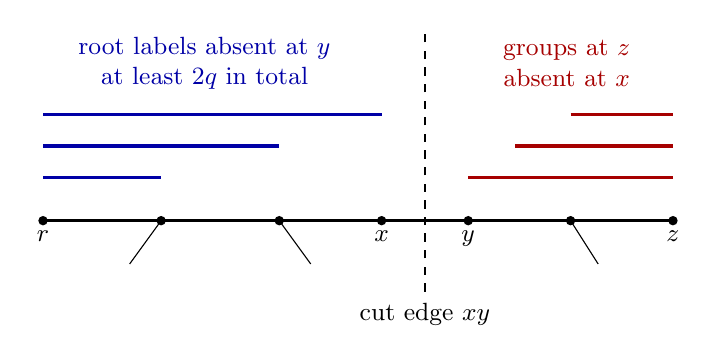
\begin{tikzpicture}[x=1cm,y=1cm,every node/.style={font=\small}]
\draw[very thick] (0,0)--(8,0);
\foreach \x in {0,1.5,3,4.3,5.4,6.7,8}
  \fill (\x,0) circle (1.7pt);
\draw (1.5,0)--(1.1,-.55);
\draw (3,0)--(3.4,-.55);
\draw (6.7,0)--(7.05,-.55);
\node[below] at (0,0) {$r$};
\node[below] at (4.3,0) {$x$};
\node[below] at (5.4,0) {$y$};
\node[below] at (8,0) {$z$};
\draw[dashed,thick] (4.85,-.9)--(4.85,2.4);
\node[below,align=center] at (4.85,-.92) {cut edge $xy$};
\draw[blue!65!black,very thick] (0,.55)--(1.5,.55);
\draw[blue!65!black,very thick] (0,.95)--(3,.95);
\draw[blue!65!black,very thick] (0,1.35)--(4.3,1.35);
\node[blue!65!black,align=center] at (2.05,2.0)
 {root labels absent at $y$\\at least $2q$ in total};
\draw[red!65!black,very thick] (5.4,.55)--(8,.55);
\draw[red!65!black,very thick] (6.0,.95)--(8,.95);
\draw[red!65!black,very thick] (6.7,1.35)--(8,1.35);
\node[red!65!black,align=center] at (6.65,2.0)
 {groups at $z$\\absent at $x$};
\end{tikzpicture}
\caption{The path argument uses cumulative absence.  The blue intervals
show intersections with the path of root subtrees that avoid \(y\);
some may end well before \(x\).  The red intervals come from group
subtrees containing \(z\) and avoiding \(x\).  The two whole families
lie on opposite sides of the cut, so no edge--vertex conflict can
occur between them.}
\label{mt:fig-path}
\end{figure}

\begin{remark}[Use with coordinate matchings]\label{mt:coordinate-interface}
In the matrix application a base label indexes at most \(s\)
coordinates, and the edge weight is the limit of the number of matched
coordinate pairs of that type divided by \(s\).  A matching gives
\eqref{mt:loads} automatically.  Deleting all pairs incident with the
fewer than \(5q\) labels missing from the common bag removes fewer
than \(5qs\) pairs.  It removes entire edge types, so any previously
chosen normalization inside a retained type stays the same.
The finite tree principle applies jointly to the original positive
label blocks and the positive blocks of the candidate edge types.
These subspaces may overlap.  A common bag consequently bounds all
their normalized Gram interactions at once.  Passing to coordinate
subsets is a compression by an isometry, so it preserves that bound.
\end{remark}
